\documentclass[12pt]{article}

%%%%%%%%%%%%%%%%%%%%%%%%%%%%%%%%%%%%%%%%%%%%%%%%%%%%%%%%%%%%%%%%%%%%%%%%%%%%%%%%
%                           Package preset for homework
%%%%%%%%%%%%%%%%%%%%%%%%%%%%%%%%%%%%%%%%%%%%%%%%%%%%%%%%%%%%%%%%%%%%%%%%%%%%%%%%
% Miscellaneous
\usepackage[margin=1in]{geometry}
\usepackage[utf8]{inputenc}
\usepackage{indentfirst}
\usepackage{blindtext}
\usepackage{graphicx}
\usepackage{xr-hyper}
\usepackage{hyperref}
\usepackage{enumitem}
\usepackage{color}
\usepackage{float}
% Math
\usepackage{latexsym}
\usepackage{amsfonts}
\usepackage{amssymb}
\usepackage{amsmath}
\usepackage{commath}
\usepackage{amsthm}
\usepackage{bbold}
\usepackage{bm}
% Physics
\usepackage{physics}
\usepackage{siunitx}
% Code typesetting
\usepackage{listings}
% Citation
\usepackage[authoryear]{natbib}
\usepackage{appendix}
\usepackage[capitalize]{cleveref}
% Title & name
\title{Homework}
\author{Tien Vo}
\date{\today}


%%%%%%%%%%%%%%%%%%%%%%%%%%%%%%%%%%%%%%%%%%%%%%%%%%%%%%%%%%%%%%%%%%%%%%%%%%%%%%%%
%                   User-defined commands and environments
%%%%%%%%%%%%%%%%%%%%%%%%%%%%%%%%%%%%%%%%%%%%%%%%%%%%%%%%%%%%%%%%%%%%%%%%%%%%%%%%
%%% Misc
\sisetup{load-configurations=abbreviations}
\newcommand{\due}[1]{\date{Due: #1}}
\newcommand{\hint}{\textit{Hint}}
\let\oldt\t
\renewcommand{\t}[1]{\text{#1}}

%%% Bold sets & abbrv
\newcommand{\N}{\mathbb{N}}
\newcommand{\Z}{\mathbb{Z}}
\newcommand{\R}{\mathbb{R}}
\newcommand{\Q}{\mathbb{Q}}
\let\oldP\P
\renewcommand{\P}{\mathbb{P}}
\newcommand{\LL}{\mathcal{L}}
\newcommand{\FF}{\mathcal{F}}
\newcommand{\HH}{\mathcal{H}}
\newcommand{\NN}{\mathcal{N}}
\newcommand{\ZZ}{\mathcal{Z}}
\newcommand{\RN}[1]{\textup{\uppercase\expandafter{\romannumeral#1}}}
\newcommand{\ua}{\uparrow}
\newcommand{\da}{\downarrow}

%%% Unit vectors
\newcommand{\xhat}{\vb{\hat{x}}}
\newcommand{\yhat}{\vb{\hat{y}}}
\newcommand{\zhat}{\vb{\hat{z}}}
\newcommand{\nhat}{\vb{\hat{n}}}
\newcommand{\rhat}{\vb{\hat{r}}}
\newcommand{\phihat}{\bm{\hat{\phi}}}
\newcommand{\thetahat}{\bm{\hat{\theta}}}

%%% Other math stuff
\providecommand{\units}[1]{\,\ensuremath{\mathrm{#1}}\xspace}
% Set new style for problem
\newtheoremstyle{problemstyle}  % <name>
        {10pt}                   % <space above>
        {10pt}                   % <space below>
        {\normalfont}           % <body font>
        {}                      % <indent amount}
        {\bfseries\itshape}     % <theorem head font>
        {\normalfont\bfseries:} % <punctuation after theorem head>
        {.5em}                  % <space after theorem head>
        {}                      % <theorem head spec (can be left empty, 
                                % meaning `normal')>

% Set problem environment
\theoremstyle{problemstyle}
\newtheorem{problemenv}{Problem}[section]
\newenvironment{problem}[1]{%
  \renewcommand\theproblemenv{#1}%
  \problemenv
}{\endproblemenv}
% Set lemma environment
\newenvironment{lemma}[2][Lemma]{\begin{trivlist}
\item[\hskip \labelsep {\bfseries #1}\hskip \labelsep {\bfseries #2.}]}{\end{trivlist}}
% Set solution environment
\newenvironment{solution}{
    \begin{proof}[Solution]$ $\par\nobreak\ignorespaces
}{\end{proof}}
\numberwithin{equation}{problemenv}

%%% Page format
\setlength{\parindent}{0.5cm}
\setlength{\oddsidemargin}{0in}
\setlength{\textwidth}{6.5in}
\setlength{\textheight}{8.8in}
\setlength{\topmargin}{0in}
\setlength{\headheight}{18pt}

%%% Code environments
\definecolor{dkgreen}{rgb}{0,0.6,0}
\definecolor{gray}{rgb}{0.5,0.5,0.5}
\definecolor{mauve}{rgb}{0.58,0,0.82}
\lstset{frame=tb,
  language=Python,
  aboveskip=3mm,
  belowskip=3mm,
  showstringspaces=false,
  columns=flexible,
  basicstyle={\small\ttfamily},
  numbers=none,
  numberstyle=\tiny\color{gray},
  keywordstyle=\color{blue},
  commentstyle=\color{dkgreen},
  stringstyle=\color{mauve},
  breaklines=true,
  breakatwhitespace=true,
  tabsize=4
}
\lstset{
  language=Mathematica,
  numbers=left,
  numberstyle=\tiny\color{gray},
  numbersep=5pt,
  breaklines=true,
  captionpos={t},
  frame={lines},
  rulecolor=\color{black},
  framerule=0.5pt,
  columns=flexible,
  tabsize=2
}


\title{Homework 4: Phys 7230 (Spring 2022)}
\due{March 14, 2022}

\begin{document}
\maketitle
%%%%%%%%%%%%%%%%%%%%%%%%%%%%%%%%%%%%%%%%%%%%%%%%%%%%%%%%%%%%%%%%%%%%%%%%%%%%%%%
\begin{problem}{1}[Variational approximation]
In the lectures we derived the classical variational bound for the free energy,
given by
\begin{equation}\label{p1:F_ineq}
    F\leq F_\t{tr}+\expval{\HH-\HH_\t{tr}}_\t{tr}, 
\end{equation}
where $H_\t{tr}$ is the variational trial Hamiltonian that best approximates
$\HH$. To prove this result we utilize the convexity of a decaying exponential
function, namely for a random variable $x$
\begin{equation}\label{p1:var_ineq}
    \expval{e^{-x}}\geq e^{-\expval{x}}. 
\end{equation}

(a) Prove above convexity inequality at least to lowest order in Taylor series
expansion.
\begin{solution}
At the limit that $x\to 0$ and $\expval{x}\to0$,
$\expval{e^{-x}}\approx\expval{1-x}=1-\expval{x}\approx e^{-\expval{x}}$. Thus,
\eqref{p1:var_ineq} is true to the lowest order in $x$ and $\expval{x}$.
\end{solution}

(b) Show that the variational inequality \eqref{p1:F_ineq} is equivalent to
$F\leq F_\t{v}=\expval{\HH}_\t{tr}-TS_\t{tr}$, where $S_\t{tr}$ is the Shannon's
entropy for the probability distribution $P=Z_\t{tr}^{-1}e^{-\beta\HH_\t{tr}}$,
with an extra factor of $k_B$ to make units consistent with our thermodynamics.
\begin{solution}
    By definition, Shannon's entropy is
\begin{align}
    S_\t{tr}
    &=-k_B\sum_q P_q\ln P_q\notag\\
    &=k_B\sum_qP_q\qty(\beta\HH_\t{tr}+\ln Z_\t{tr})\notag\\
    &=\frac1T\sum_q\HH_\t{tr}P_q+k_B\ln Z_\t{tr}\sum_q P_q\tag{$Z_\t{tr}=$
    const}\\
    &=\frac1T\expval{\HH_\t{tr}}_\t{tr}-\frac1TF_\t{tr}.
\end{align}
Thus, rearranging, we get $F_\t{tr}+\expval{\HH-\HH_\t{tr}}_\t{tr}
=\expval{\HH}_\t{tr}+F_\t{tr}-\expval{\HH_\t{tr}}_\t{tr}
=\expval{\HH}_\t{tr}-TS_\t{tr}$, as desired.
\end{solution}

(c) Consider a particle in a periodic potential described by a Hamiltonian
\begin{equation}
    \HH=\frac{p^2}{2m}+\alpha(1-\cos x), 
\end{equation}
where I took $x$ to be dimensionless, i.e., measured in units of another length
$x_0$ to simplify the notation. Motivated by the physical expectation that at
low $T$, a particle that starts at $x=0$ may be trapped in the minimum of the
cosine, use $\HH_\t{tr}=(1/2)kx^2$ to treat this problem variationally.

Specifically, please use the variational procedure to get an implicit equation
for the variational parameter function $k(\alpha/k_BT)$. Then solve this
equation for the function $k(\alpha/k_BT)$ numerically and/or graphically,
giving its two limits, the critical value of $(\alpha/k_BT)_c$ at which the
transition occurs, and sketching the function. You will find Mathematica useful.

\textit{Hint}: (1) You will find our Gaussian integral calculus very useful. (2)
You will obtain an implicit equation for the variational parameter $k$. You can
solve this equation numerically or graphically finding the behavior of
$k(\alpha/k_BT)$. From this solution show that the variational theory predicts a
phase transition in this problem in the solution for $k$ as a function of
$\alpha/k_BT$, namely that the thermodynamics (free energy, etc) has two
distinct phases, corresponding to high and low $\alpha/k_BT$. Just for the
record, this intriguing finding is an example of a failure of the variational
approximation for this single particle (0d) problem, that will, however, become
correct for higher dimensional problem, e.g., an extended $d$-dimensional
u($d>1$) object, e.g., a fluctuating membrane trapped in a periodic potential.
\begin{solution}
Let $\HH_\t{tr}=p^2/2m+(1/2)kx^2$. Then the trial partition function
is
\begin{equation}
    Z_\t{tr}=\int\frac{dxdp}{2\pi\hbar}\exp\qty(-\frac12\frac{\beta}{m}p^2
    -\frac12\beta kx^2)=\frac{k_BT}{\hbar\omega_0},
\end{equation}
where $\omega_0^2=k/m$. Then $F_\t{tr}=-k_BT\ln Z_\t{tr}$ and
$\expval{\HH_\t{tr}}_\t{tr}=k_BT$, by partition theorem on $\HH_\t{tr}$ (2
quadratic degrees of freedom). Also,
\begin{align}
    \expval{\HH}_\t{tr}
    &=\expval{\frac{p^2}{2m}}+\alpha-\alpha\expval{\cos(x/x_0)}\notag\\
    &=\frac{k_BT}{2}+\alpha-\frac{\alpha\omega_0}{2\pi k_BT}
    \sqrt{\frac{2\pi}{\beta/m}}\int_{-\infty}^\infty
    dx\cos(x/x_0)\exp\qty(-\frac12\beta kx^2)\notag\\
    &=\frac{k_BT}{2}+\alpha\qty[1-\frac{1}{\sqrt{2\pi}}
    \int_{-\infty}^\infty
        du\cos\qty(\frac{u}{x_0\sqrt{\beta k}})e^{-u^2/2}]
        \tag{$u=\sqrt{\beta k}x$}\\
    &=\frac{k_BT}{2}+\alpha\qty[1-\exp\qty(-\frac{k_BT}{2kx_0^2})].
\end{align}
Thus, the variational free energy is
\begin{align}
    F_\t{v}(k)=\expval{\HH}_\t{tr}+F_\t{tr}-\expval{\HH_\t{tr}}_\t{tr}
    =-\frac{k_BT}{2}+\alpha\qty[1-\exp\qty(-\frac{k_BT}{2kx_0^2})]-k_BT\ln\qty(\frac{k_BT}{\hbar\omega_0}).
\end{align}
In normalized units,
\begin{equation}
    \frac{F_v(k)}{k_BT}=-\frac12+\frac{\alpha}{k_BT}\qty[1-\exp\qty(-\frac{k_BT}{2kx_0^2})]-\ln\qty(\frac{k_BT}{\hbar\omega_0}). 
\end{equation}
Now, the spring constant $k$ minimizing $F_\t{v}$ satisfies $\partial
F_\t{v}(k)/\partial k=0$, which results in the following transcendental equation
\begin{equation}\label{p1c:alpha}
    \frac{\alpha}{k_BT}=\frac{kx_0^2}{k_BT}\exp\qty(\frac{k_BT}{2kx_0^2})
    =2E_0\exp\qty(\frac1{4E_0})=f(E_0),
\end{equation}
where $\alpha/k_BT$ determines the amplitude of the periodic potential, and
$E_0=(1/2)kx_0^2$ is the spring potential energy. In the following, we plot
$f(E_0)$.
\begin{center}
    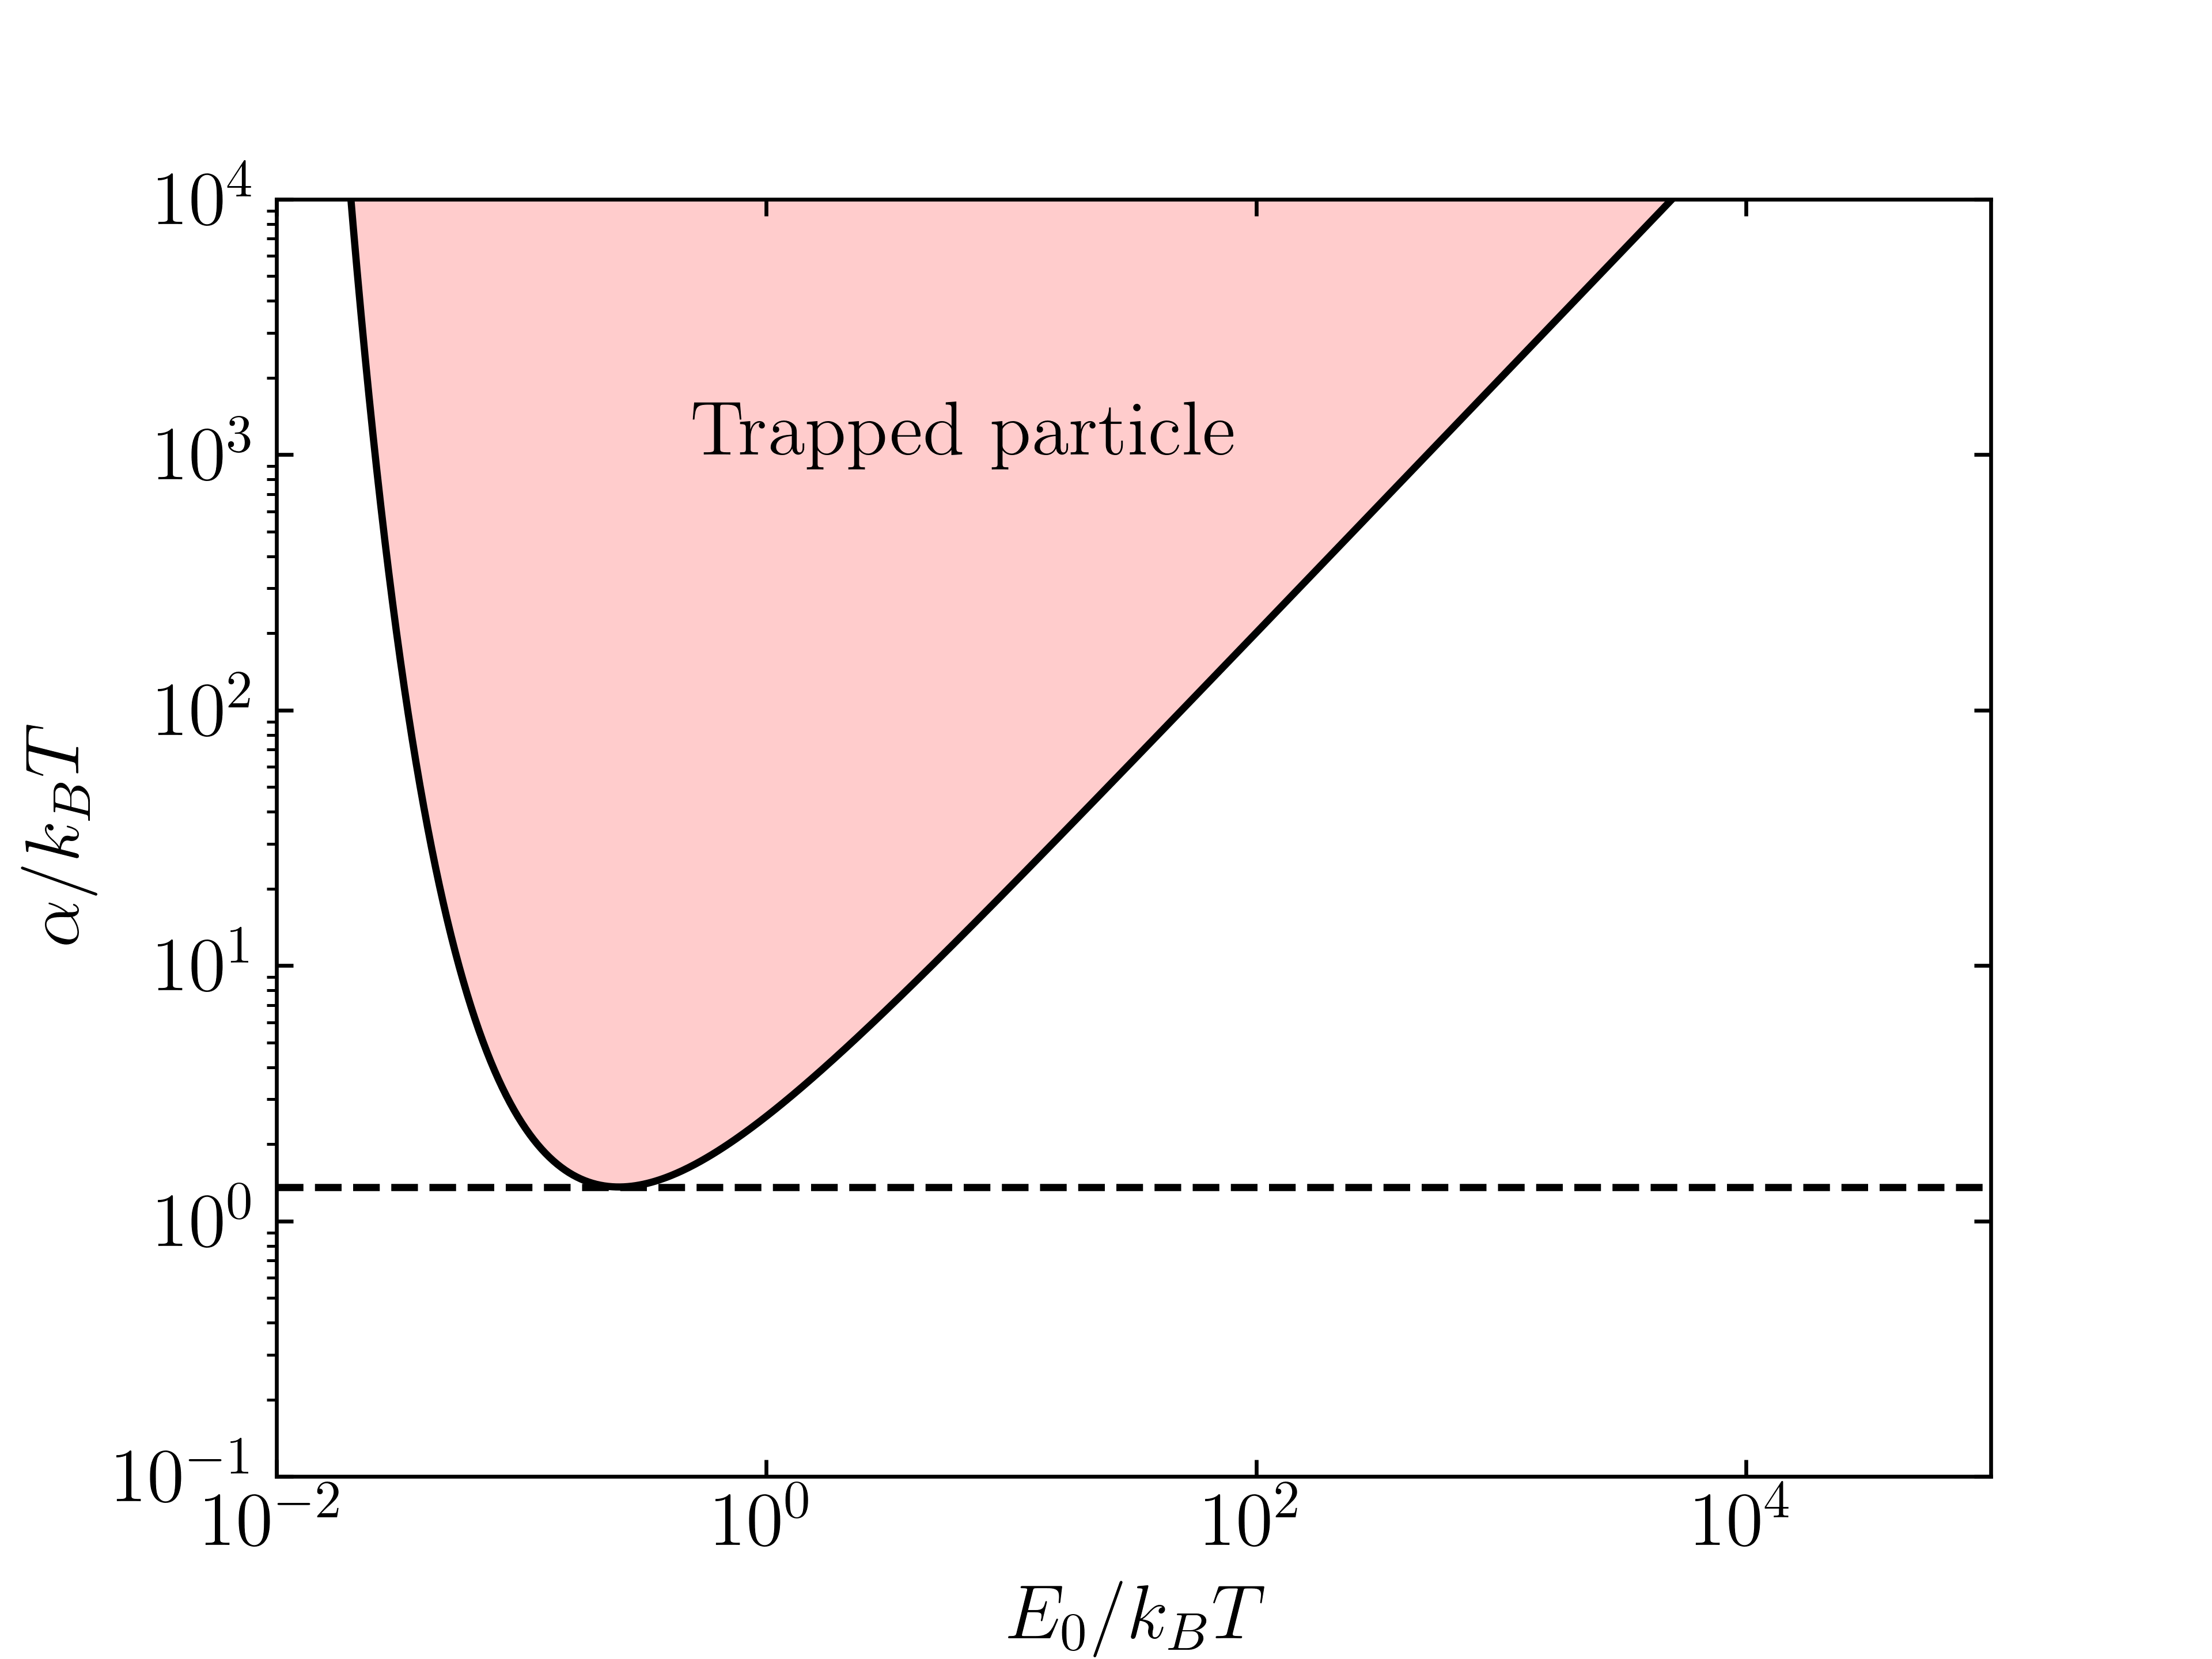
\includegraphics[width=0.8\textwidth]{p1c_1.png} 
\end{center}
For $\alpha/k_BT\lesssim1$, the potential is too small compared to the thermal
motion of the particle, not being able to trap it. When $\alpha/k_BT\gtrsim1$, 
there exists a range of $E_0$ (shaded red) in which the particle follows
harmonic motion described by $\HH_\t{tr}$. The horizontal dashed line marks the
critical value of $\alpha/k_BT\sim1.5$ and $E_0/k_BT\sim 0.2$ where this phase 
transition occurs. Furthermore, we can define the degeneracy temperature
$k_BT_\ast=4\pi^2\hbar^2/2mx_0^2$ and rewrite the variational free energy as
\begin{align}
    \frac{F_v(k_m)}{k_BT}
    &=-\frac12+\frac{\alpha}{k_BT}\qty[1-\exp\qty(-\frac{k_BT}{2kx_0^2})]
    -\ln\qty(\pi\sqrt{\frac{T/T_\ast}{E_0}})\notag\\
    &=-\frac12+2E_0\qty(e^{1/4E_0}-1)-\ln\qty(\pi\sqrt{\frac{T/T_\ast}{E_0}}),
\end{align}
where $k_m$ is the solution of \eqref{p1c:alpha}. Below, we overlay $F_v/k_BT$
onto the previous plot from $T/T_\ast=10^{-4}$ (blue) to $T/T_\ast=10^4$ (red).
Note that $F_v(k_m)/k_BT$ is only valid for $\alpha/k_BT\gtrsim1$. A low $T$
particle (blue) has significant free energy for all $E_0$, while a high $T$
particle (red) only has significant free energy for low $E_0$ or high $E_0$.
\begin{center}
    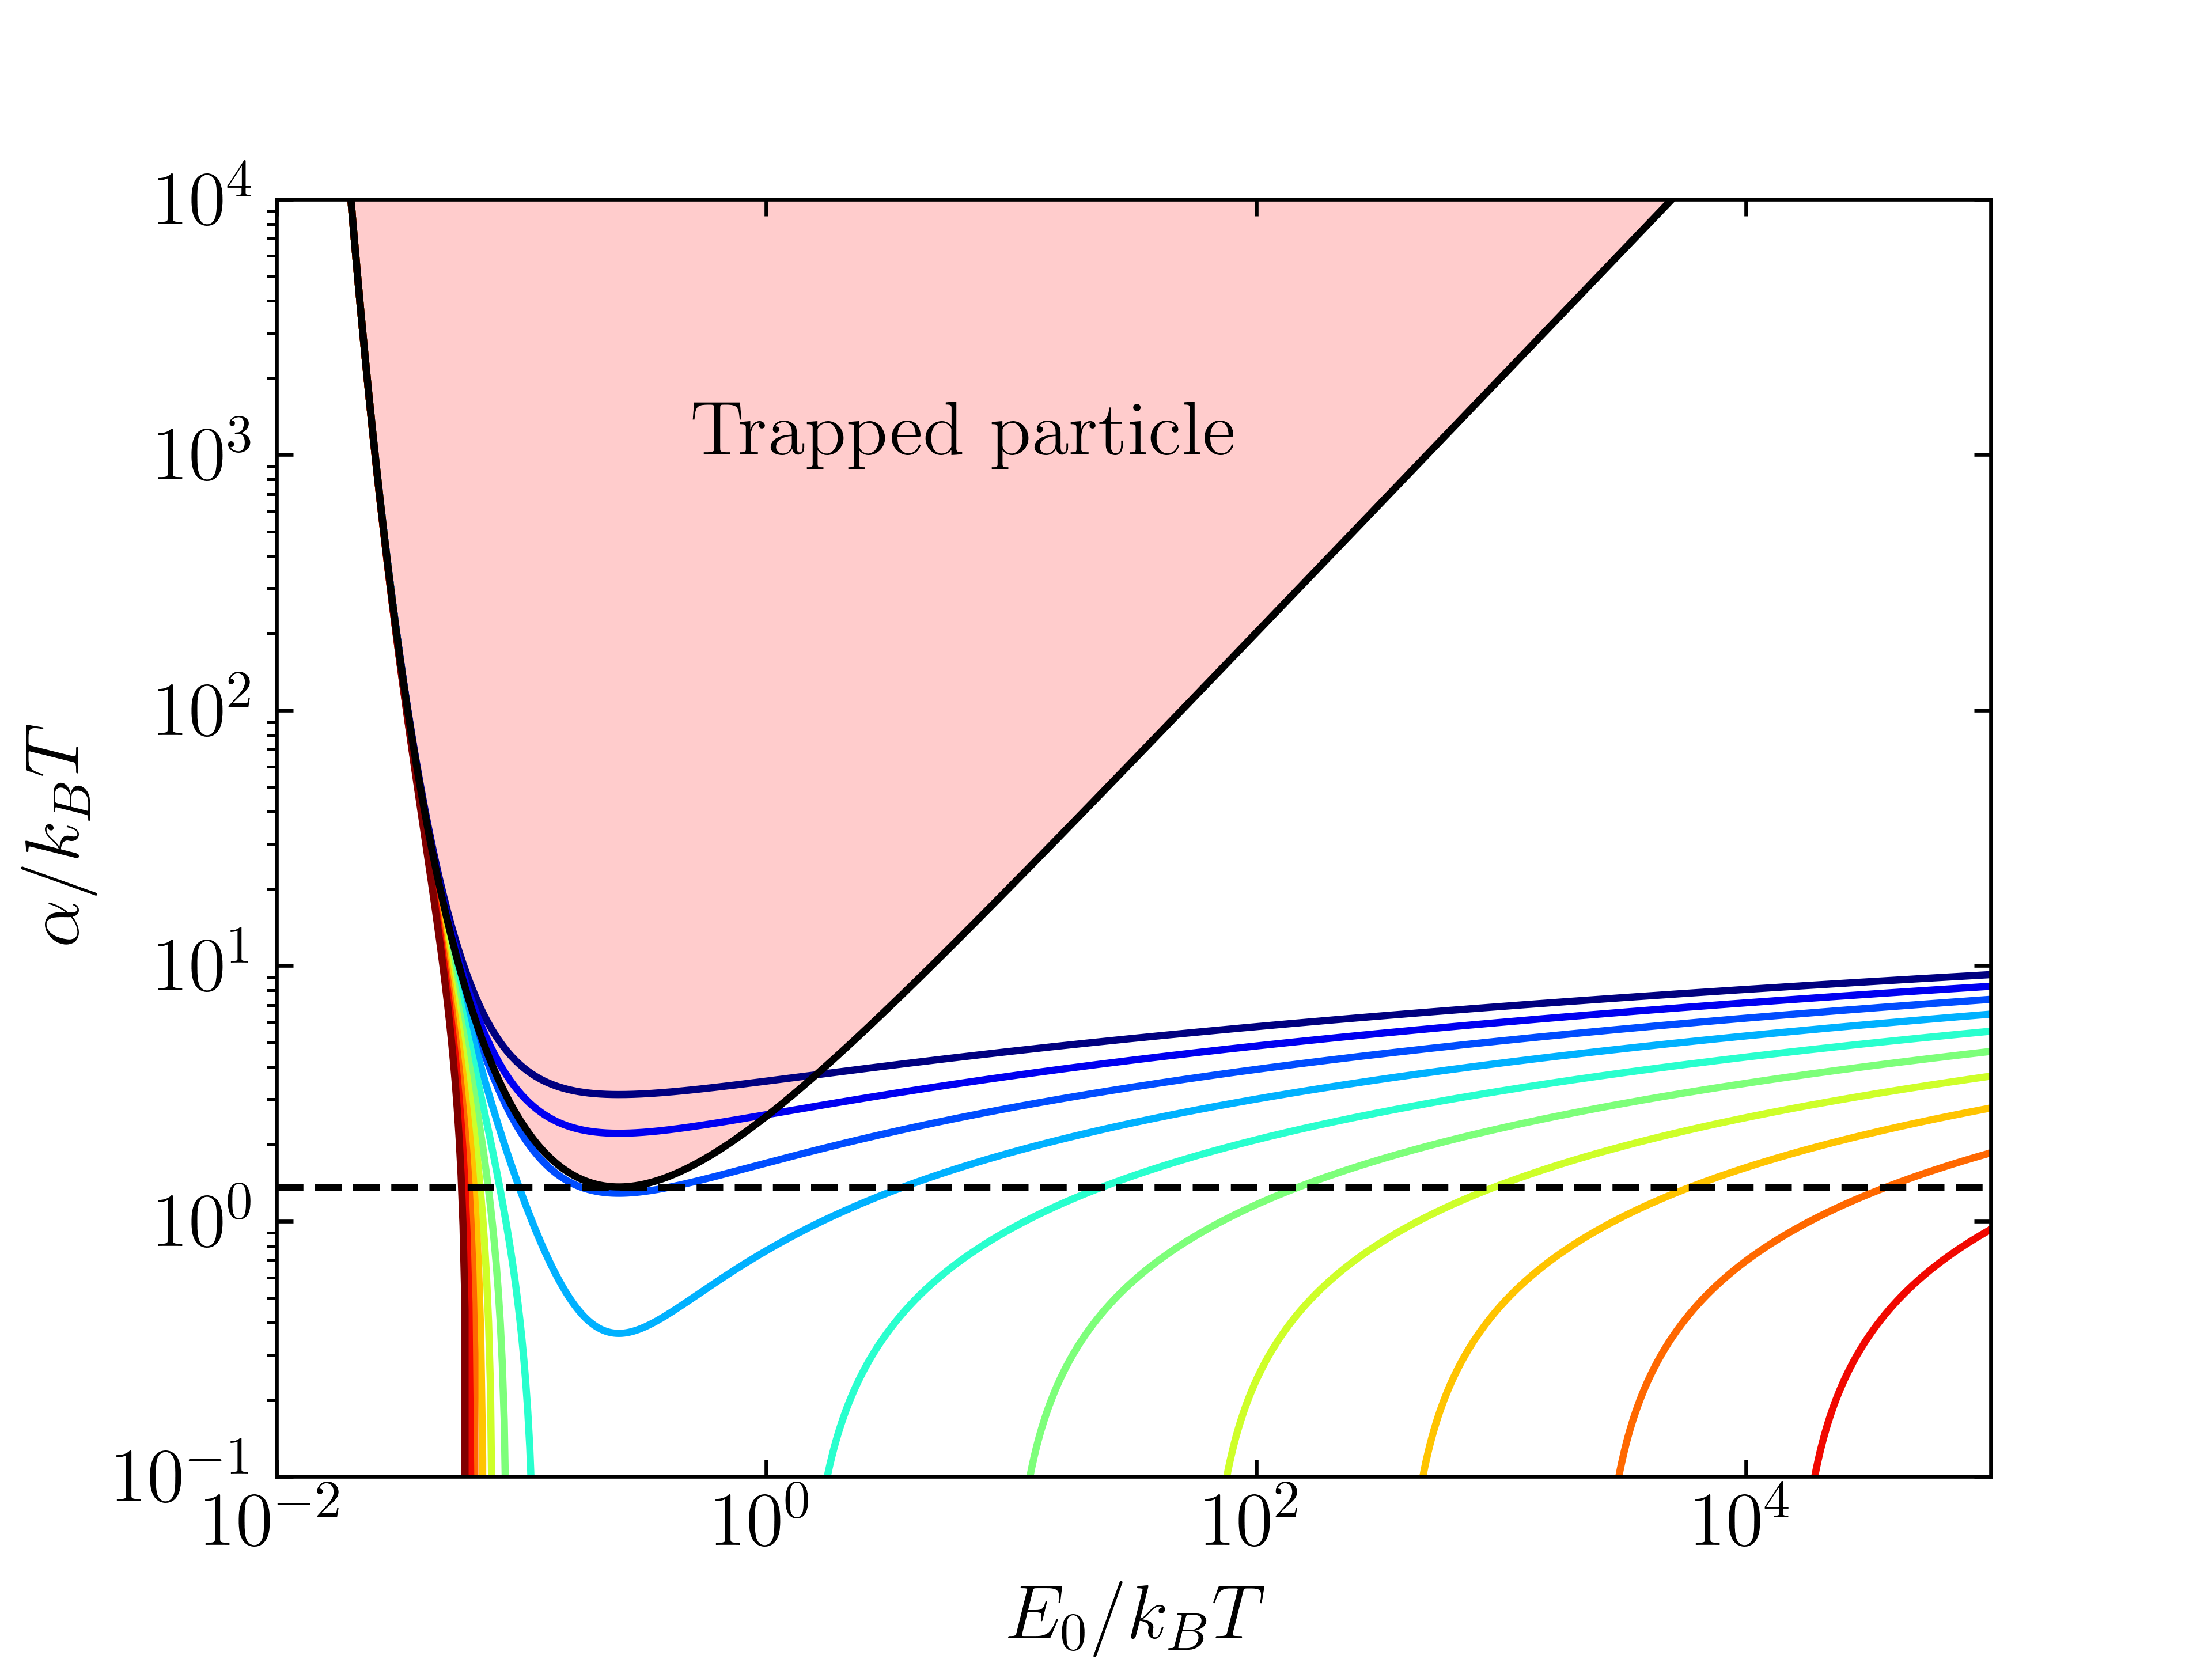
\includegraphics[width=0.8\textwidth]{p1c_2.png} 
\end{center}
\end{solution}
\end{problem}
\newpage
%%%%%%%%%%%%%%%%%%%%%%%%%%%%%%%%%%%%%%%%%%%%%%%%%%%%%%%%%%%%%%%%%%%%%%%%%%%%%%%    

%%%%%%%%%%%%%%%%%%%%%%%%%%%%%%%%%%%%%%%%%%%%%%%%%%%%%%%%%%%%%%%%%%%%%%%%%%%%%%%
\begin{problem}{2}[Propagation in imaginary time, random walk and phantom
    polymer]

(a) Using Gaussian integral calculus demonstrate an important and very useful
(e.g., for path integrals and our applications below) Gaussians ``propagation''
relation,
\begin{equation}\label{p2a:prop_rel}
    \int_{-\infty}^\infty
    dx_2\frac1{\sqrt{2\pi\tau_2}}e^{-\frac{(x_3-x_2)^2}{2\tau_2}}
    \frac1{\sqrt{2\pi\tau_1}}e^{-\frac{(x_2-x_1)^2}{2\tau_1}}
    =\frac1{\sqrt{2\pi(\tau_2+\tau_1)}}e^{-\frac{(x_3-x_1)^2}{2(\tau_2+\tau_1)}},
\end{equation}
and thereby prove unnormalized density matrix the ``propagator'' property for
the \textit{free-particle},
\begin{equation}\label{p2a:prop_property}
    \rho^u(x_3,x_1;\tau_1+\tau_2)
    =\int dx_2\rho^u(x_3,x_2;\tau_2)\rho^u(x_2,x_1;\tau_1),
\end{equation}
that, as discussed in class is satisfied by all $\rho^u(x,x',\tau)$.
\begin{solution}
From the LHS of \eqref{p2a:prop_rel},
\begin{align}
    \t{LHS}
    &=\frac1{2\pi\sqrt{\tau_1\tau_2}}\int_{-\infty}^\infty dx_2
    \exp\qty[-\frac{(x_3-x_2)^2}{2\tau_2}-\frac{(x_2-x_1)^2}{2\tau_1}]\notag\\
    &=\frac1{2\pi\sqrt{\tau_1\tau_2}}\exp\qty[-\frac{x_3^2\tau_1+x_1^2\tau_2}{2\tau_1\tau_2}]
    \int_{-\infty}^\infty
    dx_2\exp\qty[-\frac12\frac{\tau_1+\tau_2}{\tau_1\tau_2}x_2^2+\frac{x_3\tau_1+x_1\tau_2}{\tau_1\tau_2}x_2]\notag\\
    &=\frac1{\sqrt{2\pi(\tau_1+\tau_2)}}\exp\qty[\frac1{2\tau_1\tau_2(\tau_1+\tau_2)}\qty(2x_1x_3\tau_1\tau_2-x_1^2\tau_1\tau_2-x_3^2\tau_1\tau_2)]\notag\\
    &=\frac1{\sqrt{2\pi(\tau_1+\tau_2)}}\exp\qty[-\frac{(x_3-x_1)^2}{2(\tau_1+\tau_2)}]\notag\\
    &=\t{RHS}.
\end{align}
Now, for a 1-d free partice, the density matrix is
\begin{align}
    \rho^u(x,x';\beta=\tau/\hbar)
    &=\frac1{\lambda_T}\exp\qty[-\pi\frac{(x-x')^2}{\lambda_T^2}]
        \tag{$\lambda_T=h\sqrt{\beta/2\pi m}$}\\
    &=\frac1{\hbar}\sqrt{\frac{m}{2\pi\beta}}
    \exp\qty[-\frac{m}{\hbar^2}\frac{(x-x')^2}{2\beta}]\notag\\
    &=\sqrt{\frac{m}{\hbar}}\frac1{\sqrt{2\pi\tau}}
        \exp\qty[-\frac{m}{\hbar}\frac{(x-x')^2}{2\tau}]\notag\\
    &=\frac{1}{\sqrt{2\pi\overline{\tau}}}
        \exp\qty[-\frac{(x-x')^2}{2\overline\tau}],
\end{align}
where we have set $\overline\tau=\tau\hbar/m$ for simplification. Then, it
follows from the RHS of \eqref{p2a:prop_property} that
\begin{align}
    \t{RHS}
    &=\int dx_2\frac1{\sqrt{2\pi\overline\tau_2}}
        \exp\qty[-\frac{(x_3-x_2)^2}{2\overline\tau_2}]
        \frac1{\sqrt{2\pi\overline\tau_1}}
        \exp\qty[-\frac{(x_2-x_1)^2}{2\overline\tau_1}]\notag\\
    &=\frac1{\sqrt{2\pi(\overline\tau_1+\overline\tau_2)}}
    \exp\qty[-\frac{(x_3-x_1)^2}{2(\overline\tau_1+\overline\tau_2)}]\notag\\
    &=\rho^u(x_3,x_1;\tau_1+\tau_2)\notag\\
    &=\t{LHS}.
\end{align}
\end{solution}

(b) Edward's ``phantom'' polymer model, coupled harmonic oscillators, and a
random walk

As we may discuss in more detail in a few lectures, a simplest model of a
polymer (a giant flexible linear molecule of $N$ monomers strung together,
illutrated in \cref{fig:p2b} below) is that of a freely-joined chain of $N$
links $\vb{r}_n=\vb{R}_n-\vb{R}_{n-1}$. In the continuum, $n\to s$, the
probability of its conformation $\vb{R}(s)$ in a $d$-dimensional space is given
by
\begin{equation}\label{p2b:P}
    P\qty[\vb{R}(s)]=\qty(\frac{d}{2\pi b_0^2})^{dN/2}
    \exp\qty[-\frac{d}{2b_0^2}\int_0^N ds\qty(\frac{\partial\vb{R}}{\partial
        s})^2],
\end{equation}
where $b_0$ is the preferred link length and prefactor is a normalization, much
like in \cref{p2a:prop_rel} for 2 links. We can view this system as described by
an ideal polymer Hamiltonian

\begin{figure}
    \centering
    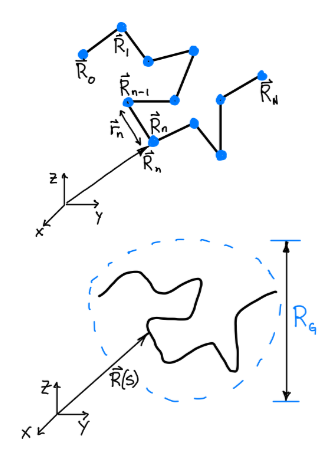
\includegraphics[width=0.4\textwidth]{p2b.png}
    \caption{Edward's ``phantom'' polymer model executing an ideal random walk
    in $d$-dimensional space, characterized by $N+1$ monomer positions,
$\vb{R}_n$.}
\label{fig:p2b}
\end{figure}

\begin{equation}
    \HH=\frac\sigma2\int_0^Nds\qty(\frac{\partial\vb{R}}{\partial s})^2,  
\end{equation}
where $\sigma=k_BTd/(\pi b_0^2)$ is the entropic polymer free energy per unit of
length, i.e., tension, notably proportional to thermal energy $k_BT$.

\qquad(i) By discretizing above probability distribution into product of $N$
1-link probability distributions,
\begin{equation}
    p(\vb{r}_n)=\qty(\frac{d}{2\pi b_0^2})^{d/2}
    \exp\qty[-\frac{d}{2b_0^2}\qty(\vb{R}_n-\vb{R}_{n-1})^2],
\end{equation}
written in terms of the position $\vb{R}_n$ of $n$-th monomer, and by
integrating over all $N$ \textit{intermediate} monomer positions, $\vb{R}_n$ for
$1<n<N$ compute the probability distribution $P\qty[\vb{R}_N-\vb{R}_0]$, for the
end-to-end displacement $\vb{R}_N-\vb{R}_0$.

\textit{Hint}: Surprise! You have just computed a path-integral for a single
polymer statistical mechanics, computing its partition function
$Z=\exp\qty(-\beta F)$, for fixed ends $\vb{R}_N,\vb{R}_0$ of the polymer.
\begin{solution}
From \eqref{p2b:P}, we discretize $\int_0^Nds\mapsto\sum_{n=1}^N$
\begin{align}
    P[\vb{R}(s)]
    &\approx\qty(\frac{d}{2\pi b_0^2})^{dN/2}
    \exp\qty[-\frac{d}{2b_0^2}\sum_{n=1}^N\qty(\vb{R}_n-\vb{R}_{n-1})^2]\notag\\
    &=\qty(\frac{d}{2\pi b_0^2})^{dN/2}
    \prod_{n=1}^N\exp\qty[-\frac{d}{2b_0^2}\qty(\vb{R}_n-\vb{R}_{n-1})^2]\notag\\
    &=\prod_{n=1}^N\qty(\frac{d}{2\pi b_0^2})^{d/2}
    \exp\qty[-\frac{d}{2b_0^2}\qty(\vb{R}_n-\vb{R}_{n-1})^2]\notag\\
    &=\prod_{n=1}^Np(\vb{r}_n).
\end{align}
Then,
\begin{align}
    P\qty[\vb{R}_N-\vb{R}_0]
    &=\int d^d\vb{R}_1\hdots d^d\vb{R}_{N-1}\prod_{n=1}^Np(\vb{r}_n)\notag\\
    &=\qty(\frac{d}{2\pi b_0^2})^{dN/2}
    \exp\qty[-\frac{d}{2b_0^2}\qty(\vb{R}_0^2+\vb{R}_N^2)]
    \int d^d\vb{R}_1\hdots d^d\vb{R}_{N-1}\notag\\
    &\qquad\times
    \exp\qty[-\frac{d}{b_0^2}\qty(\vb{R}_1^2-\vb{R}_0\vdot\vb{R}_1
        +\vb{R}_2^2-\vb{R}_1\vdot\vb{R}_2+\hdots
        +\vb{R}_{N-1}^2-\vb{R}_{N}\vdot\vb{R}_{N-1})]\notag\\
    &=\qty(\frac{d}{2\pi b_0^2})^{dN/2}
        \exp\qty[-\frac{d}{2b_0^2}\qty(\vb{R}_0^2+\vb{R}_N^2)]
        \int d\vb{u}\exp\qty[-\frac{d}{b_0^2}
        \qty(\vb{u}^T\vdot\vb{A}\vdot\vb{u}-\vb{h}^T\vdot\vb{u})],
\end{align}
where $\vb{u}=\mqty(\vb{R}_1&\hdots&\vb{R}_{N-1})^T$,
$\vb{h}=\mqty(\vb{R}_0&\hdots&\vb{R}_N)^T$ are $d(N-1)$-dimensional vectors.
\begin{equation}
    \vb{A}
    =\mqty(
        \mathbb{1} & -(1/2)\mathbb{1} & \hdots & 0 & 0\\
        (-1/2)\mathbb{1} & \mathbb{1} & -(1/2)\mathbb{1} & \hdots & 0\\
        \vdots  &   -(1/2)\mathbb{1}  &   \ddots  &   \ddots  &   \vdots\\
        0 & 0 & \ddots & \mathbb{1} & -(1/2)\mathbb{1}\\
        0 & 0 & \hdots & -(1/2)\mathbb{1} & \mathbb{1}
    )
\end{equation}
is a symmetric block matrix of $d$-dimensional identity matrices $\mathbb{1}$. 
By Gaussian integration that we derived in Homework 2,
\begin{align}
    Z_0=\int
    d\vb{u}\exp\qty[-\frac12\frac{2d}{b_0^2}\vb{u}^T\vdot\vb{A}\vdot\vb{u}]
    =\frac1{\qty(\det\vb{A})^{d/2}}\qty(\frac{\pi b_0^2}{d})^{d(N-1)/2},
\end{align}
where $\det\vb{A}=N/2^{N-1}$, by construction and note the power of $d$ in the
determinant comes from the fact that it is a block matrix. Now, we also need to 
calculate
\begin{align}
    \frac{d}{4b_0^2}\vb{h}^T\vdot\vb{A}^{-1}\vdot\vb{h} 
    &=\frac{d}{4b_0^2}\qty(A_{1,1}^{-1}\vb{R}_0^2+2\vb{A}_{1,N-1}^{-1}\vb{R}_0\vdot\vb{R}_N+A_{N-1,N-1}^{-1}\vb{R}_N^2).
\end{align}
The inverse of $\vb{A}$ is defined as $\vb{A}^{-1}=\t{cof}(\vb{A})/\det\vb{A}$
where $\t{cof}(\vb{A})$ is the cofactor matrix of $\vb{A}$ with elements defined
by
\begin{align}
    \qty(\t{cof}A)_{i,j}=(-1)^{i+j}\det\vb{A}_{ij},
\end{align}
where $\vb{A}_{ij}$ is the $i,j$ \textit{minor} of $\vb{A}$, not the $i,j$
element. Thus,
\begin{equation}
    A_{1,1}^{-1}=A_{N-1,N-1}^{-1}=\frac2N(N-1),\qquad\t{and}
    \qquad
    A_{1,N-1}^{-1}=\frac2N.
\end{equation}
Putting all of this together, we can finally write the probability distribution
function of $\vb{R}_N-\vb{R}_0$ as
\begin{align}
    P\qty[\vb{R}_N-\vb{R}_0]
    &=\qty(\frac{d}{2\pi b_0^2})^{dN/2}
        \exp\qty[-\frac{d}{2b_0^2}\qty(\vb{R}_0^2+\vb{R}_N^2)]
        \frac{2^{d(N-1)/2}}{N^{d/2}}\qty(\frac{\pi b_0^2}{d})^{d(N-1)/2}
        \notag\\
    &\qquad\times
        \exp\qty[\frac{d}{2b_0^2N}\qty[(N-1)(\vb{R}_0^2+\vb{R}_N^2)+2\vb{R}_0\vdot\vb{R}_N]]\notag\\
    &=\qty(\frac{d}{2\pi b_0^2N})^{d/2}
        \exp\qty[-\frac{d}{2b_0^2N}(\vb{R}_N-\vb{R}_0)^2],
\end{align}
which resembles the 1-link PDF.
\end{solution}

\qquad(ii) Compute the ``radius of gyration'' $R_g(N)$, defined by
\begin{equation}
    R_g^2=\expval{\qty(\vb{R}_N-\vb{R}_0)^2}, 
\end{equation}
which characterizes the root-mean-squared radius occupied by a polymer in the
$d$-dimensional embedding space.

Note that, in thinking of the links of the polymer as random steps executed as a
function of ``time'' $s$, this polymer statistics reproduces the random walk
result that after $N$ steps the random walker is only $\sqrt{N}$ away from where
she started. All this is of course a consequence of central limit theorem.

\begin{solution}
Let $\vb{X}=\vb{R}_N-\vb{R}_0$, then
\begin{align}
    R_g^2=\expval{\vb{X}^2} 
    &=\qty(\frac{d}{2\pi b_0^2N})^{d/2}
    \int d^d\vb{X} \exp\qty[-\frac12\frac{d}{b_0^2N}\vb{X}^2]\vb{X}^2\notag\\
    &=\qty(\frac{d}{2\pi b_0^2N})^{d/2}
    \prod_{i=1}^d\qty[\int_{-\infty}^\infty dX_i\qty(\sum_{j=1}^dX_j^2)
    \exp\qty(-\frac12\frac{d}{b_0^2N}X_i^2)]\notag\\
    &=\qty(\frac{d}{2\pi b_0^2N})^{d/2}\sqrt{\frac{(2\pi)^{d-1}}{d/b_0^2N}}
    \frac1{d/b_0^2N}\sqrt{\frac{2\pi}{d/b_0^2N}}\notag\\
    &=b_0^2\frac{N}{d}.
\end{align}
Thus, $R_g$ indeed grows as $\sqrt{N}$.
\end{solution}
\end{problem}
\newpage
%%%%%%%%%%%%%%%%%%%%%%%%%%%%%%%%%%%%%%%%%%%%%%%%%%%%%%%%%%%%%%%%%%%%%%%%%%%%%%%
%%%%%%%%%%%%%%%%%%%%%%%%%%%%%%%%%%%%%%%%%%%%%%%%%%%%%%%%%%%%%%%%%%%%%%%%%%%%%%%
\begin{problem}{3}[Free particle density matrix in coordinate representation]
In lectures we discussed many properties and forms of the coordinate-space
density matrix $\rho(x,x';\beta)$, including its expected low- and high-$T$
limits, as well as its eigenstates
\begin{equation}\label{p3:H_basis}
    \rho^u(x,x';\beta)=\sum_n\psi_n(x)\psi_n^\ast(x')e^{-\beta E_n},
\end{equation}
and path-integral
\begin{equation}\label{p3:path_int}
    \rho^u(x,x';\beta)=\int_{x(0)=x;x(\beta\hbar)=x'}\qty[dx(\tau)]
    e^{-S_E\qty[x(\tau)]/\hbar}
\end{equation}
formulations, as well as the ``imaginary-time'' Schr\"{o}dinger-like equation in
$\beta$
\begin{equation}\label{p3:Schrodinger_eq}
    \partial_\beta\rho^u(x,x';\beta)=-\HH\qty(\hat\rho,x)\rho^u(x,x';\beta), 
\end{equation}
that it satisfies, where $\hat\rho=-i\hbar\partial_x$, i.e., giving the
coordinate representation Schr\"{o}dinger equation in imaginary time. Let us
explore the details of this for a free particle here.

(a) For a free particle, use its Hamiltonian inside \eqref{p3:Schrodinger_eq},
solve the resulting diffusion equation (in ``time'' $\beta$) solve, taking into
account the appropriate ``initial condition''  for $\beta=0$, discussed in
class, required by the general definition of $\hat\rho^u$.

\textit{Hint}: The solution is as simple as solving free-particle
Schr\"{o}dinger equation in imaginary ``time'' or a real diffusion equation in
infinite space.
\begin{solution}
First, by separation of variables, we write
$\rho(x,x';\beta)=X(\vb{x},\vb{x}')B(\beta)$. Then from
\eqref{p3:Schrodinger_eq},
\begin{align}
    \frac{1}{B}\frac{dB}{d\beta}=\frac{\hbar^2}{2m}\frac1{X}\grad^2X
    =-E,
\end{align}
where $E$ is some constant. This separates into two ordinary differential
equations in $\vb{x}$ and $\beta$, in which the general solutions are
$B=e^{-\beta E}$ and
\begin{equation}
    X(x,x')=f(\vb{k})\sin\qty(\vb{k}\vdot\vb{x})+
    g(\vb{k})\cos\qty(\vb{k}\vdot\vb{x}),
\end{equation}
where $E=\hbar^2k^2/2m$. However, by normalization condition,
$\rho(\vb{x},\vb{x},\beta=0)=1$, so we must require $f(\vb{k})=0$. The general 
solution for $\rho$ is then a linear combination of these basis functions
\begin{equation}
    \rho(\vb{x},\vb{x}';\beta)
    =\int d^d\vb{k}
        g(\vb{k})\cos(\vb{k}\vdot\vb{x}) e^{-\beta \hbar^2k^2/2m}.
\end{equation}
Now, note that for $\beta\to0$ and $\vb{x},\vb{x}'\in\R^d$,
\begin{equation}
    \rho(\vb{x},\vb{x}';\beta=0)
    =\int d^d\vb{k}g(\vb{k})\cos(\vb{k}\vdot\vb{x})
    =\delta(\vb{x}-\vb{x}')=\frac1{\qty(2\pi)^d}\int
    d^d\vb{k}e^{i\vb{k}\vdot(\vb{x}-\vb{x}')}.
\end{equation}
Thus, we can solve for $g(\vb{k})$ and write the final solution as
\begin{align}
    \rho(\vb{x},\vb{x}';\beta) 
    &=\frac1{2\pi}\int d^d\vb{k}\exp\qty[-\frac12\frac{\beta\hbar^2}{m}k^2
    +i\qty(\vb{x}-\vb{x}')\vdot\vb{k}]\notag\\
    &=\frac1{\qty(2\pi)^d}\qty(\frac{2\pi}{\beta\hbar^2/m})^{d/2}
    \exp\qty[-\frac{(\vb{x}-\vb{x}')^2}{2\beta\hbar^2/m}]\notag\\
    &=\qty(\frac{m}{2\pi\hbar^2\beta})^{d/2}
    \exp\qty[-\frac12\frac{m(\vb{x}-\vb{x}')^2}{\hbar^2\beta}].
\end{align}
\end{solution}

(b) Use Hamiltonian eigenbasis representation, \cref{p3:H_basis} and your
knowledge of what the free-particle eigenstates are, to rederive the above
result for $\rho^u(x,x';\beta),$ also quoted in the lectures. Note that if you
properly take the eigenstates to be normalized in a large box of size $L$ (most
convenient with periodic boundary conditions), this analysis automatically gives
the correct prefactor for $\rho^u(x,x';\beta)$.
\begin{solution}
The eigenstate of a particle in an infinite square well for
$x\in\qty[-L/2,L/2]$ is
\begin{equation}
    \psi_n(x)=\sqrt{\frac2L}\sin\qty[\frac{n\pi x}{2}+\frac{n\pi}{2}],
\end{equation}
with energy $E_n=n^2\pi^2\hbar^2/2mL^2$. Thus, from \eqref{p3:H_basis},
\begin{align}
    \rho(x,x';\beta)
    =\frac2L\sum_{n=0}^\infty \sin\qty[\frac{n\pi x}{L}+\frac{n\pi}{2}]
    \sin\qty[\frac{n\pi x'}{L}+\frac{n\pi}{2}]
    \exp\qty[-\beta\frac{n^2\pi^2\hbar^2}{2m L^2}].
\end{align}
Letting $\sum_{n}\mapsto\sum_0^\infty dn$, we can calculate this infinite series
with Mathematica
\begin{align}
    \rho\qty(x,x';\beta)
    =\sqrt{\frac{m}{2\pi\hbar^2\beta}}
    \qty{\exp\qty[-\frac12\frac{m(x-x')^2}{\hbar^2\beta}]
    -\exp\qty[-\frac12\frac{m(L+x+x')^2}{\hbar^2\beta}]}.
\end{align}
Thus, taking the limit that $L\to\infty$, the second exponent vanishes, leaving
the 1-dimensional form of the answer in part (a).
\end{solution}

(c) Now we will use, perhaps a bit less familiar path-integral formulation. One
useful approach to evaluate a path-integral is that of a semi-classical
saddle-point approximation.

\begin{itemize}
    \item An amazing fact, however, that we will see below is that this
        semi-classical approach is in fact \textit{exact} for a quadratic
        action, as for e.g.,, a free particle and harmonic oscillator (the
        following problem).
    \item Examining \cref{p3:path_int}, we see that all dependence of
        $\rho^u(x,x';\beta)$ on $x,x'$ is in the boundary conditions on
        $x(0),x(\beta\hbar)$. So let's introduce new time-dependent coordinates
        $y(\tau)$, with
        \begin{equation}\label{p3c:new_x}
            x(\tau)=x_\t{cl}(\tau)+y(\tau), 
        \end{equation}
        where $x_\t{cl}(\tau)$ is the classical path satisfying the
        Euler-Lagrange equation
        \begin{equation}\label{p3c:eom}
            \eval{\frac{\delta S_E\qty[x(\tau)]}{\delta
            x(\tau)}}_{x_\t{cl}(\tau)}=0, 
        \end{equation}
        and satisfying $x_\t{cl}(0)=x,x_\t{cl}(\beta\hbar)=x'$. Thus,
        $y(0)=y(\beta\hbar)=0$.

    \item Inserting \cref{p3c:new_x} into the action in \cref{p3:path_int} and
        expanding to lowest nontrivial order in $y(\tau)$ we find
        \begin{equation}\label{p3c:approx_dens_matrix}
            \rho^u(x,x';\beta)\approx
            e^{-S_E\qty[x_\t{cl}(\tau)]/\hbar}
            \int_{y(0)=y(\beta\hbar)=0}\qty[dy(\tau)]
            \exp\qty[-\frac1{2\hbar}\int_0^{\beta\hbar}d\tau
            y(\tau)S_E''[x_\t{cl}]y(\tau)],
        \end{equation}
        where first functional derivative term is absent because it vanishes by
        virtue of the equation of motion \cref{p3c:eom} satisfied by 
        $x_\t{cl}(\tau)$.

    \item The key observation in \cref{p3c:approx_dens_matrix} is that for
        quadratic action $S_E\qty[x(\tau)]$, the kernel $S_E''\qty[x_\t{cl}]$
        in the exponential is independent of $x_\t{cl}(\tau)$. Thus, for such
        quadratic theory, the remaining functional integral over
        $y(\tau)\NN(\beta\hbar)$ is just a ``constant'' that only depends on
        $\beta\hbar$, but \textit{not} not on $x,x'$. We can therefore not worry
        about this prefactor $\NN(\beta\hbar)$ and focus on
        $\exp\qty(-S_E\qty[x_\t{cl}(\tau)]/\hbar)$ that contains all the key
        dependence on $x,x'$, giving us $\rho^u(x,x';\beta)$ up to the factor
        $\NN(\beta\hbar)$.
\end{itemize}

\begin{solution}
    See part (d).
\end{solution}

(d) For a free particle, solve the (Euclidean) classical Euler-Lagrange equation
of motion \cref{p3c:eom} for $x(\tau,x,x')$ with initial conditions
$x_\t{cl}(0)=x,x_\t{cl}(\beta\hbar)=x'$, and evaluate
\begin{equation}
    S_E\qty[x_\t{cl}(\tau)]\equiv S_\t{cl}(x,x',\beta\hbar), 
\end{equation}
thereby obtaining
\begin{equation}\label{p3d:dens_matrix}
    \rho^u(x,x';\beta)=\NN(\beta\hbar)e^{-S_\t{cl}(x,x',\beta\hbar)/\hbar}. 
\end{equation}
Demonstrate that up to the unknown prefactor $\NN(\beta\hbar)$, you obtain
exactly the result found in (a) and (b).
\begin{solution}
    The Lagrangian of a free particle is $\LL=(1/2)m\dot{x}^2$. Thus, the action is 
$S_E[x(\tau)]=(m/2)\int_0^{\beta\hbar}d\tau\dot{x}^2$. Then it follows that
\begin{align}
    \frac{\delta S_E[x(\tau)]}{\delta x(\tau)}
    &=\lim_{\epsilon\to0}\frac1\epsilon\qty{S_E\qty[x(t)+\epsilon\delta(t-\tau)]-S_E[x(t)]}\notag\\
    &=\frac{m}{2}\int_0^{\beta\hbar}dt\lim_{\epsilon\to0}\frac1\epsilon
    \qty{\qty[\dot{x}+\epsilon\delta'(t-\tau)]^2-\dot{x}^2}\notag\\
    &=\frac{m}{2}\int_0^{\beta\hbar}dt\lim_{\epsilon\to0}
    \qty[2\dot{x}\delta'(t-\tau)+\epsilon\delta'^2]\notag\\
    &=m\int_0^{\beta\hbar}\dot{x}\delta'(t-\tau)\notag\\
    &=-m\ddot{x}.
\end{align}
Extremizing $S_E$, it follows that the classical trajectory
is $x_\t{cl}(\tau)=a\tau+b$ for some constant
$a,b\in\R$. Now, using the initial conditions $x_\t{cl}(0)=x$ and
$x_\t{cl}(\beta\hbar)=x'$, we can write
\begin{equation}
    x_\t{cl}(\tau)=-\frac{x-x'}{\beta\hbar}\tau+x .
\end{equation}
Then, from \eqref{p3c:approx_dens_matrix},
\begin{align}
    \rho^u(x,x';\beta)
    &\approx \NN(\beta\hbar)\exp\qty[-\frac{S_E[x_\t{cl}(\tau)]}{\hbar}]\notag\\
    &=\NN(\beta\hbar)\exp\qty[-\frac{m}{2}\frac{(x-x')^2}{\beta^2\hbar^3}\int_0^{\beta\hbar}d\tau]\notag\\
    &=\NN(\beta\hbar)\exp\qty[-\frac12\frac{m(x-x')^2}{\hbar^2\beta}],
\end{align}
which is the same as previous results, up to a factor $\NN(\beta\hbar)$.   
\end{solution}

(e) As a non-required bonus, you can determine the prefactor $\NN(\beta\hbar)$,
by discretizing the path integral in \eqref{p3c:approx_dens_matrix} as you did
for a polymer in problem 2 (note mathematically it is exactly the same path
integral) and then requiring the $\NN(\Delta\tau)$ (with
$\beta\hbar=N\Delta\tau)$ to be special function such that the ``propagator''
relation, \eqref{p2a:prop_rel} is satisfied.

Alternatively,you can determine $\NN(\tau)$ by requiring that
\eqref{p3d:dens_matrix} satisfies the diffusion equation,
\eqref{p3:Schrodinger_eq}, thereby obtaining and solving a differential equation
for $\NN(\tau)$.
\begin{solution}
\end{solution}

(f) Now that we have obtained $\rho^u(x,x';\beta)$ by three methods above,
calculate the corresponding (i) partition function $Z(\beta)$ and the (ii)
probability $P(x)=\rho^u(x,x,\beta)/Z(\beta)$ of finding a free particle at
position $x$.

\textit{Hint}: The answer makes sense and is trivial.
\begin{solution}
(i) By definition, the partition function $Z$ is the trace
\begin{equation}
    Z=\int
    d\vb{x}\rho(\vb{x},\vb{x};\beta)=\qty(\frac{m}{2\pi\hbar^2\beta})^{d/2}\int
    d\vb{x}.
\end{equation}
Viewing the free particle as a particle in a large infinite square well, if the 
domain is $[-L,L]^d$ for $L\to\infty$, then $Z\to\infty$ as well and
(ii) it follows that $P(x)\to\infty$. Mathematically, this makes sense because
the continuous probability distribution function $P(\vb{x})=\rho/Z$ is 
infinitely dense. So the probability is only non-zero in any non-zero measure
subset of the support of $P$ ($\qty{\vb{x}}$ is a zero measure set).

But physically, it is due to equilibriation. Diffusion in an infinite space 
with the ergodicity hypothesis blows up the uncertainty in $x$. But we know 
precisely the momentum (or energy). Now, this would no longer be true for finite
$L$, in which the energy eigenvalues are discretized. So the probability in this
limit may be finite and equates to
\begin{equation}
    P(\vb{x})=\frac1{V(L)}\exp\qty[-\frac{m(\vb{x}-\vb{x}')^2}{2m\hbar^2\beta}],
\end{equation}
where $V=\int_{[-L,L]^d}d\vb{x}$ is the volume of the square well.
\end{solution}

\end{problem}
\newpage
%%%%%%%%%%%%%%%%%%%%%%%%%%%%%%%%%%%%%%%%%%%%%%%%%%%%%%%%%%%%%%%%%%%%%%%%%%%%%%%
%%%%%%%%%%%%%%%%%%%%%%%%%%%%%%%%%%%%%%%%%%%%%%%%%%%%%%%%%%%%%%%%%%%%%%%%%%%%%%%
\begin{problem}{4}[Particle in harmonic potential density matrix in coordinate
    representation]

Here we want to calculate $\rho^u(x,x',\beta)$ and the corresponding partition
function $Z$ and $P(x)$ for a quantum harmonic oscillator. The first two methods
(a) and (b), above are in fact a bit challenging to utilize, though the solution
of the imaginary-time Schr\"{o}dinger equation (a) is quite straightforward, but
technically grungy. So below we will focus on the path-integral approach.

Carefully following the path-integral procedure in problem 3, above, now for a
quantum harmonic oscilator.

(a) Calculate $\rho^u(x,x';\beta)$ from the path-integral analysis, by finding
$x_\t{cl}(\tau)$ and the corresponding
$S_E\qty[x_\t{cl}(\tau)]=S_\t{cl}(x,x',\beta\hbar)$, and using
\eqref{p3d:dens_matrix}, up to a prefactor $\NN(\beta\hbar)$.
\begin{solution}
The Lagrangian is $\LL=(1/2)m\dot{x}^2-(1/2)m\omega_0^2x^2$ where
$\omega_0^2=k/m$. Thus, the E-L equation of motion is
\begin{equation}
    m\ddot{x}=\frac{\partial\LL}{\partial x}
    =-m\omega_0^2x\Rightarrow\frac{d^2x}{dt^2}=-\omega_0^2x
    \Rightarrow\frac{d^2x}{d\tau^2}=\omega_0^2x,
\end{equation}
where we have writte $t=-i\tau$. The general solution to this differential
equation is
\begin{equation}
    x(\tau)=Ae^{\omega_0\tau}+Be^{-\omega_0\tau}, 
\end{equation}
where
\begin{equation}
    A=\frac{x-e^{\beta\hbar\omega_0}x'}{1-e^{2\beta\hbar\omega_0}},\qquad\t{and}
    \qquad
    B=-e^{\beta\hbar\omega_0}\frac{e^{\beta\hbar\omega_0}x-x'}{1-e^{2\beta\hbar\omega_0}}
\end{equation}
satisfy the initial conditions $x(0)=x,x(\beta\hbar)=x'$. It follows that the
unnormalized density matrix is
\begin{align}
    \rho^u(x,x';\beta)
    &=\NN(\beta\hbar)\exp\qty[-\frac{m}{2\hbar}\int_0^{\beta\hbar}d\tau\qty(\dot{x}^2-\omega_0^2x^2)]\notag\\
    &=\NN\exp\qty[\frac{m}{2\hbar}\int_0^{\beta\hbar}d\tau
    \qty((dx/d\tau)^2+\omega_0^2x^2)]\notag\\
    &=\NN\exp\qty[-\frac{m\omega_0}{2\hbar}
        \qty[A^2\qty(1-e^{2\beta\hbar\omega_0})-B^2\qty(1-e^{-2\beta\hbar\omega_0})]]\notag\\
    &=\NN\exp\qty[-\frac{m\omega_0}{4\hbar}\qty[(x+x')\tanh\qty(\frac{\beta\hbar\omega_0}{2})+(x-x')^2\coth\qty(\frac{\beta\hbar\omega_0}{2})]]
\end{align}
\end{solution}

(b) Compute the canonical partition function $Z$ (that you have done in an
earlier homework) to determine the prefactor $\NN(\beta\hbar)$.
\begin{solution}
The Hamiltonian is $\HH=p^2/2m+(1/2)m\omega_0^2x^2$ with eigenvalues
$E_n=\hbar\omega_0(n+1/2)$. Thus, the partition function is
\begin{align}
    Z=\sum_{n=0}^\infty\exp\qty[-\beta\hbar\omega_0\qty(n+\frac12)]
    =e^{-\beta\hbar\omega_0/2}\sum_{n=0}^\infty\qty(e^{-\beta\hbar\omega_0})^n
    =\frac1{2\sinh\qty(\beta\hbar\omega_0/2)}.
\end{align}
But the trace of $\rho^u$ is also $Z$
\begin{align}
    Z=\NN\int_{-\infty}^\infty dx
    \exp\qty[-\frac{m\omega_0}{\hbar}\tanh\qty(\frac{\beta\hbar\omega_0}{2})x^2]
    =\NN\sqrt{\frac{\pi\hbar}{m\omega_0\tanh(\beta\hbar\omega_0/2)}}.
\end{align}
Thus,
\begin{equation}
    \NN=\frac1{2\sinh\qty(\beta\hbar\omega_0/2)}\sqrt{\frac{m\omega_0\tanh(\beta\hbar\omega_0/2)}{\pi\hbar}}
    =\sqrt{\frac{m\omega_0}{2\pi\hbar\sinh\qty(\beta\hbar\omega_0)}}.
\end{equation}
\end{solution}

(c) Compute the probability density
$P(x)=\rho^u(x,x,\beta)/Z(\beta)=\rho(x,x,\beta)$ of finding the particle in a
harmonic potential at position $x$.
\begin{solution}
From previous results,
\begin{align}
    P(x)=\frac{\rho^u}{Z}
    =\sqrt{\frac{m\omega_0\tanh(\beta\hbar\omega_0/2)}{\pi\hbar}}\exp
    \qty(-\frac{m\omega_0\tanh(\beta\hbar\omega_0/2)}{\hbar}x^2).
\end{align}
\end{solution}

(d) Using $P(x)$, compute the root-mean-squared length $x_Q(T)$, defined by the
variance $x_Q^2(T)=\expval{x^2}$.
\begin{solution}
By definition,
\begin{align}
    &&x_Q^2
    &=\sqrt{\frac{m\omega_0\tanh(\beta\hbar\omega_0/2)}{\pi\hbar}}
    \int_{-\infty}^\infty dx
    x^2\exp\qty(-\frac{m\omega_0\tanh(\beta\hbar\omega_0/2)}{\hbar}x^2)\notag\\
    &&&=\frac{\hbar}{2m\omega_0\tanh(\beta\hbar\omega_0/2)}.\notag\\
    &\Rightarrow&
    x_Q&=\sqrt{\frac{\hbar}{2m\omega_0\tanh(\beta\hbar\omega_0/2)}}.
\end{align}
\end{solution}

(e) Study high- and low-temperature limits of $x_Q(T)$, and make arguments for
the resulting limiting forms, by thinking about the purely classical and purely
quantum limits of the harmonic oscillator.
\begin{solution}
Let the crossover temperature be $T_\ast=\hbar\omega_0/k_B$ and
$x_0=\hbar/m\omega_0$ such that the maximum spring potential energy is exactly
one quantum of energy $(1/2)kx_0^2=\hbar\omega_0/2$. Then $x_Q$ can be rewritten
as
\begin{equation}
   x_Q=x_0\frac1{\sqrt{2\tanh\qty(T^\ast/2T)}} .
\end{equation}
Below, we plot this function.
\begin{center}
    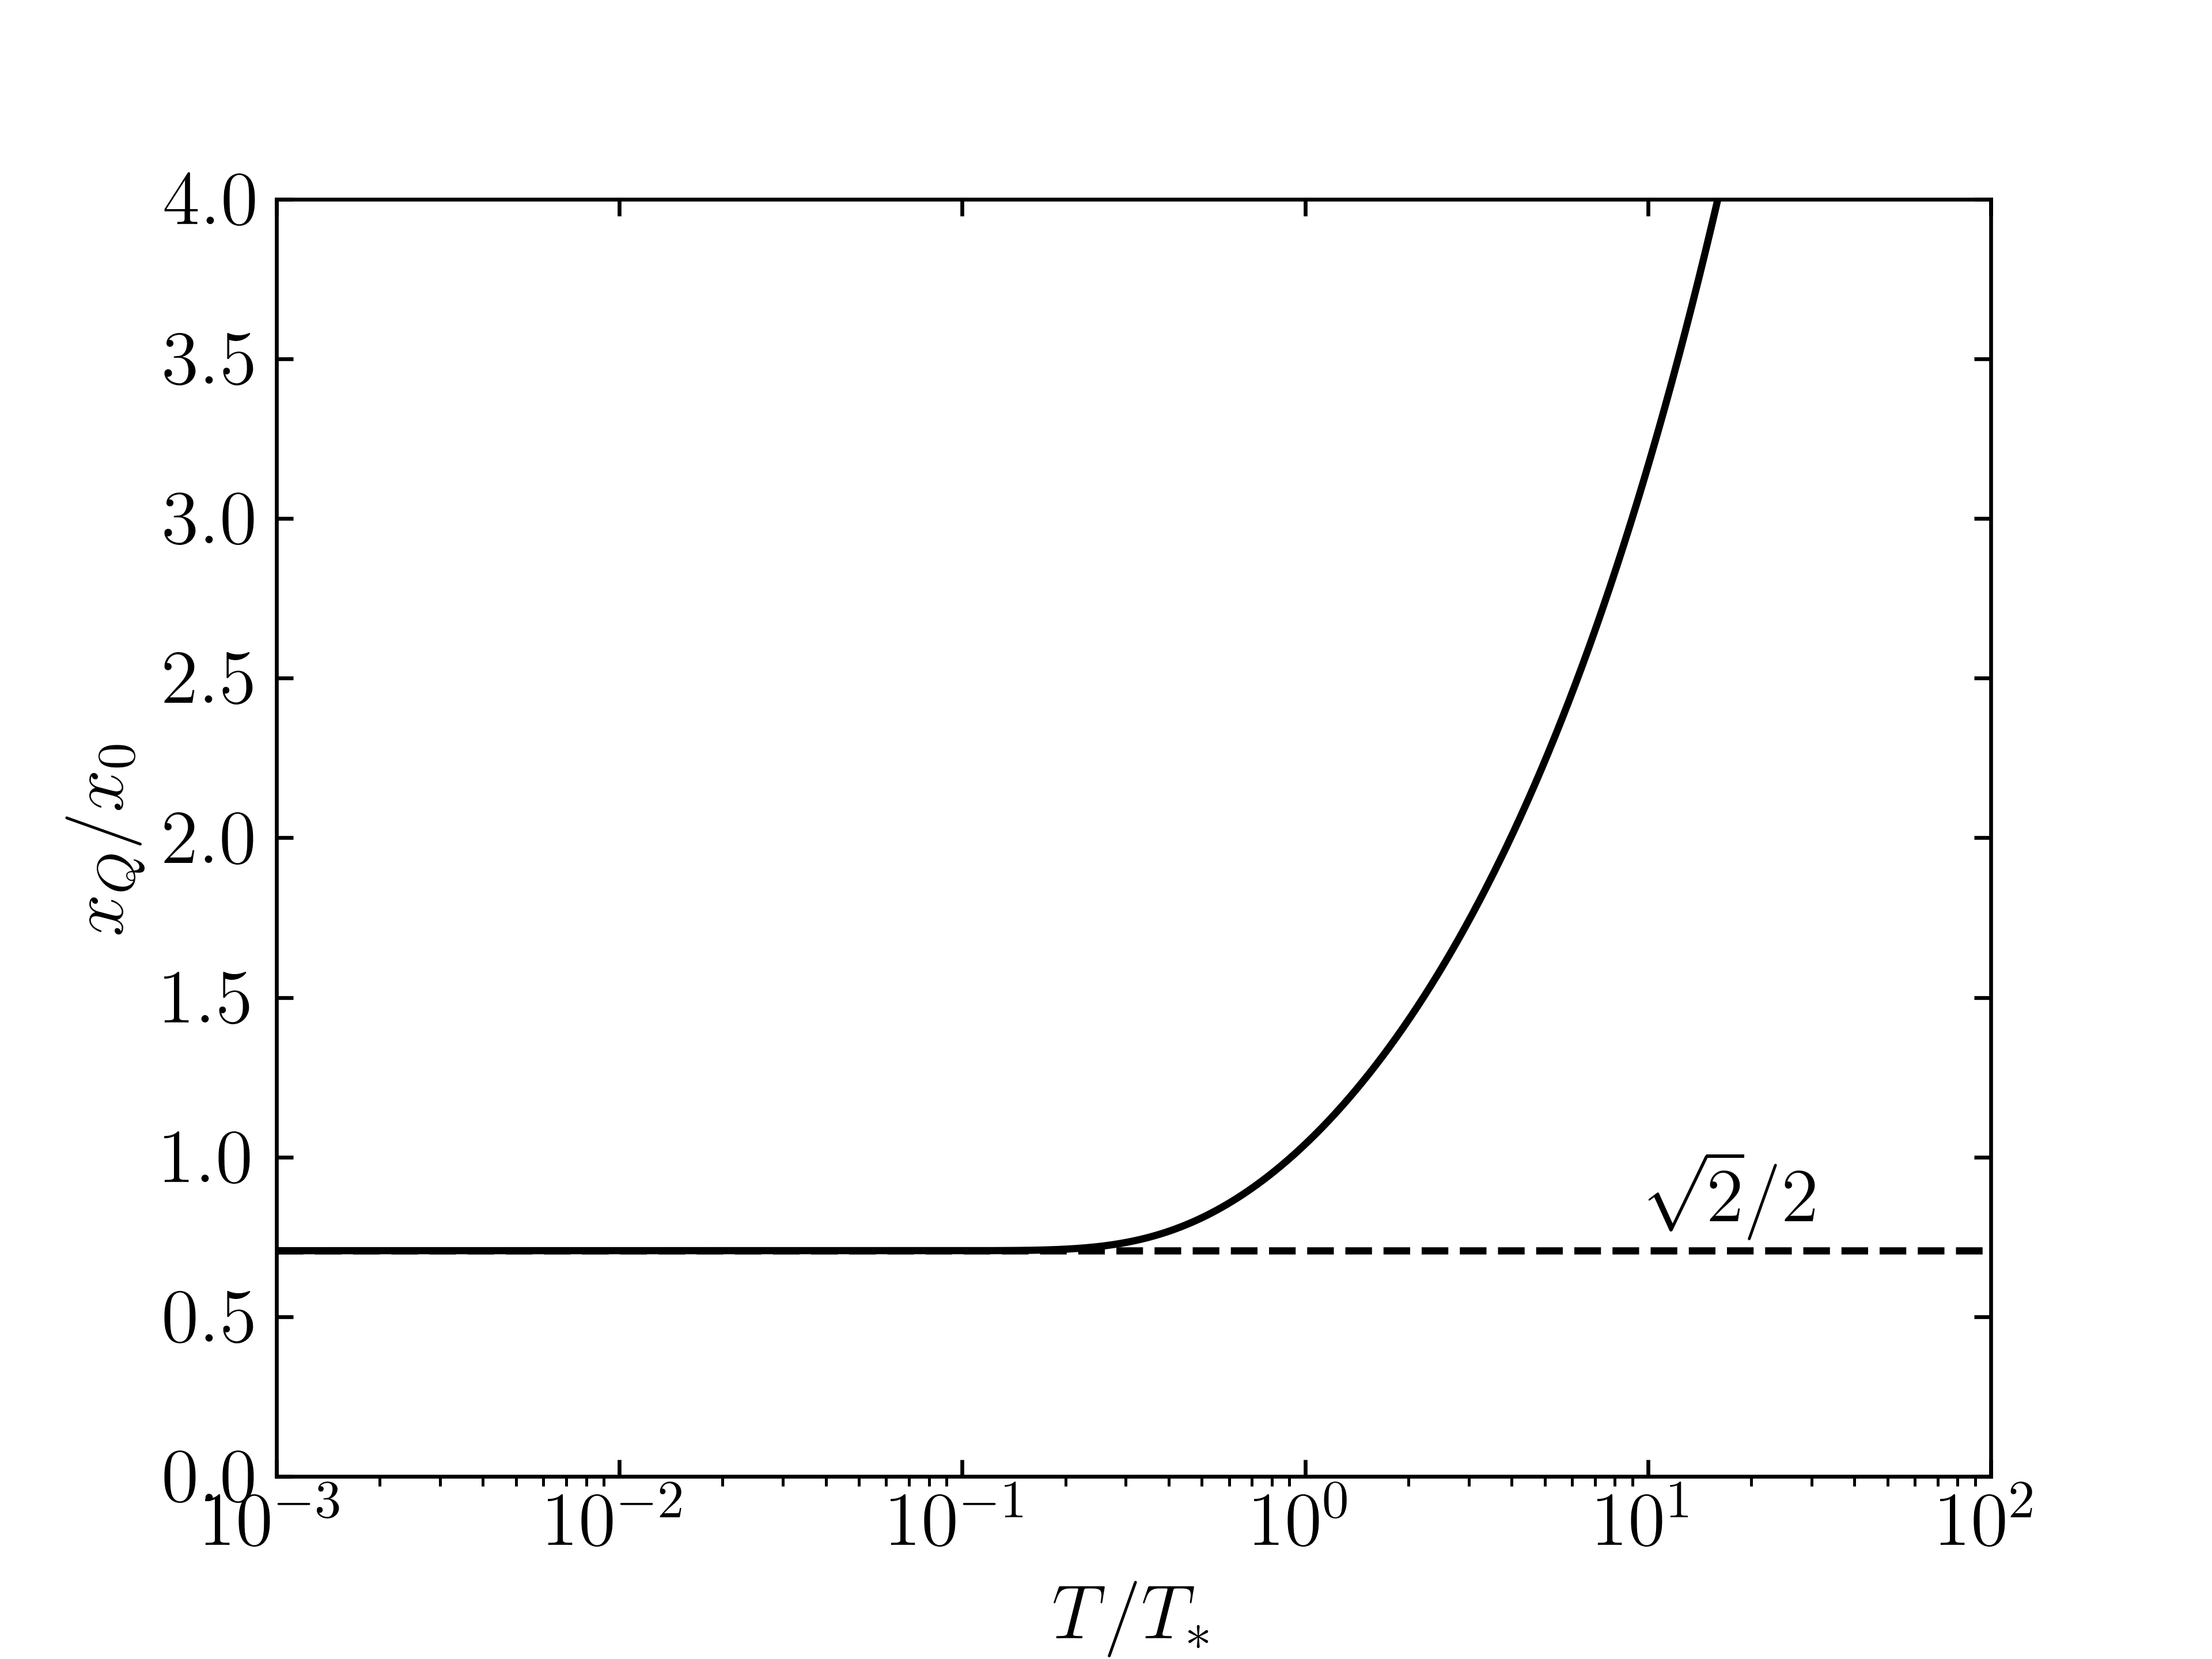
\includegraphics[width=0.8\textwidth]{p4.png} 
\end{center}
In the low temperature limit ($T/T_\ast\ll 1$), $x_Q$ approaches the limit
of $x_0/\sqrt2$. Recall the time-dependent solution of
a harmonic oscillator $x\sim x_0e^{i\omega_0t}$. Thus
$\expval{x^2}=x_0^2\expval{e^{i\omega_0t}}=x_0^2/2$. So this limit makes sense.
In the classical regime ($T/T_\ast\gg1$), the available energy is much larger
than $\hbar\omega_0/2$. Also, the scale of the oscillation in $x$ is much larger
than that defined by the quantum scale $x_0$. So it makes sense that
$x_Q\to\infty$.
\end{solution}
\end{problem}
\newpage
%%%%%%%%%%%%%%%%%%%%%%%%%%%%%%%%%%%%%%%%%%%%%%%%%%%%%%%%%%%%%%%%%%%%%%%%%%%%%%%
%%%%%%%%%%%%%%%%%%%%%%%%%%%%%%%%%%%%%%%%%%%%%%%%%%%%%%%%%%%%%%%%%%%%%%%%%%%%%%%
\begin{problem}{5}[Density matrix and entanglement entropy]
Consider a system consisting of two qubits (``quantum bit'', each realized as
any two-level system e.g., a double-well potential or a spin-1/2 or just two
atomic levels, a basic element of a quantum computer) $A$ and $B$, with each
taking on two possible values, designated by, say 0 and 1. Take this 2-qubit
``computer'' to be in a pure

(a) \textit{unentangled}, i.e., product state
\begin{equation}
    \ket{\psi_{AB}}=\frac12\qty(\ket{0}+\ket1)\otimes\qty(\ket0+\ket1).
\end{equation}

Construct the two-qubit density matrix
$\hat\rho_{AB}=\ket{\psi_{AB}}\bra{\psi_{AB}}$ for the whole system and extract
its corresponding ($4\times4$) matrix representation $\rho_{ss'}$ in this
$\ket{s}=\ket{\sigma_A}\otimes\ket{\sigma_B}$ ($\sigma_{A,B}=0,1\mapsto
s=1,2,3,4$) basis, namely
$\hat\rho_{AB}=\sum_{s,s'=1}^4\rho_{ss'}\ket{s}\bra{s'}=\sum_{\sigma,\sigma'=0,1}\rho_{ss'}\ket{\sigma_A}\otimes\ket{\sigma_{B}}\bra{\sigma_A'}\otimes\bra{\sigma_B'}$.

\qquad(i) Verify that this is indeed a density matrix for a pure state by
showing $\Tr[\hat\rho_{AB}]=\Tr[\hat\rho_{AB}^2]=1$. \textit{Hint}: You can do 
this by working directly with the matrix $\rho_{\sigma\sigma'}$ or more 
formally working in a representation-independent way.
\begin{solution}
First, we write $\ket{1}=\ket{0,0},\ket{2}=\ket{0,1},\ket{3}=\ket{1,0},$ and
$\ket{4}=\ket{1,1}$. Now, by assumption,
\begin{align}\label{p5a:psi}
    \ket{\psi_{AB}}\bra{\psi_{AB}}
    &=\frac14\qty(\ket{0,0}+\ket{0,1}+\ket{1,0}+\ket{1,1})
    \qty(\bra{0,0}+\bra{0,1}+\bra{1,0}+\bra{1,1})\notag\\
    &=\frac14\qty(\ket{1}+\ket{2}+\ket{3}+\ket{4})\qty(\ket{1}+\ket{2}+\ket{3}+\ket{4}).
\end{align}
Reading off directly from this, we can write the density matrix as
\begin{equation}
    \hat{\rho}_{AB}=\frac14\mqty(1&1&1&1\\1&1&1&1\\1&1&1&1\\1&1&1&1),
    \qquad\t{and}\qquad
    \hat{\rho}_{AB}^2=\hat{\rho}_{AB}
    =\frac14\mqty(1&1&1&1\\1&1&1&1\\1&1&1&1\\1&1&1&1).
\end{equation}
Thus, by definition, the trace is the sum of the diagonals and it is obvious
that $\Tr[\hat\rho_{AB}]=\Tr[\hat\rho_{AB}^2]=1$.
\end{solution}

\qquad(ii) Show that the von Neumann entropy of this state vanishes, i.e.,
\begin{equation}
    S_{vN}=-\expval{\ln\hat\rho_{AB}}=-\Tr\qty(\hat\rho_{AB}\ln\hat\rho_{AB})=0, 
\end{equation}
as it must for any pure state. \textit{Hint}: One way to define a function of an
operator (e.g., $\ln\hat{O}$) is by its eigenvalues by going to its diagonal
basis.
\begin{solution}
We diagonalize $\hat\rho_{AB}$ by finding the roots of
$\det\mqty(\hat\rho_{AB}-\sigma\mathbb{1})=\sigma^4-\sigma^3=\sigma^3\qty(\sigma-1)$,
which are 0 and 1. Thus indeed,
\begin{equation}
    S_{vN}=-\Tr\qty[\hat\rho_{AB}\ln\hat\rho_{AB}]
    =-\sum_{\sigma=0,1}\sigma\ln\sigma=0.
\end{equation}
\end{solution}

\qquad(iii) Compute the reduced ($2\times2$) density matrix
\begin{equation}
    \hat\rho_A=\Tr\hat\rho_{AB}=\sum_{\sigma_B}\ev{\hat\rho_{AB}}{\sigma_B},
\end{equation}
by tracing over the states of the $B$ qubit, that describes the density matrix
for the $A$ qubit subsystem.
\begin{solution}
From \eqref{p5a:psi}, we find that
\begin{equation}
    \mel{0}{\hat\rho_{AB}}{0}
    =\mel{0}{\hat\rho_{AB}}{1}
    =\mel{1}{\hat\rho_{AB}}{0}
    =\mel{1}{\hat\rho_{AB}}{1}
    =\frac14\qty[\ket{0}+\ket{1}]\qty[\bra{0}+\bra{1}]
    =\frac12.
\end{equation}
Thus,
\begin{equation}
    \hat\rho_A=\frac12\mqty(1&1\\1&1),\qquad\t{and}\qquad
    \hat\rho_A^2=\frac12\mqty(1&1\\1&1).
\end{equation}
\end{solution}

\qquad(iv) Verify that this reduced density matrix describes a pure state, by
showing $\Tr[\hat\rho_A]=\Tr[\hat\rho_A^2]=1$.
\begin{solution}
The trace is just the sum of the diagonal elements, which is 1 for both,
obviously. 
\end{solution}

\qquad(v) Show that consistent with above, the \textit{entanglement} entropy
(von Neumann entropy of $\hat\rho_A$) for subsystem $A$, described by this
reduced density matrix, $\hat\rho_A$ still vanishes, i.e.,
\begin{equation}
    S_E=-\expval{\ln\hat\rho_A}_A=-\Tr\qty(\hat\rho_A\ln\hat\rho_A)=0, 
\end{equation}
demonstrating that the qubits $A$ and $B$ are not entangled, since
$\hat\rho_{AB}$ was constructed from a \textit{product} state.
\begin{solution}
    Again we find the eigenvalues from the roots of
    $\det\qty(\hat\rho_A-\sigma_A\mathbb{1})=\lambda(\lambda-1)$, which are
    still 0 and 1. Thus, $S_E=-\sum_{\sigma_A=0,1}\sigma_A\ln\sigma_A=0$.
\end{solution}

(b) \textit{entangled} ``cat'' state
\begin{equation}
    \bra{\psi_{AB}}=\frac1{\sqrt2}\qty(\ket0\otimes\ket0+\ket1\otimes\ket1).
\end{equation}
Construct the two-qubit density matrix
$\hat\rho_{AB}=\ket{\psi_{AB}}\bra{\psi_{AB}}$ for the whole system and extract
its corresponding ($4\times4$) matrix representation $\rho_{ss'}$ in this
$\ket{s}=\ket{\sigma_A}\otimes\ket{\sigma_B}$ ($\sigma_{A,B}=0,1\mapsto
s=1,2,3,4$) basis, namely
$\hat\rho_{AB}=\sum_{s,s'=1}^4\rho_{ss'}\ket{s}\bra{s'}=\sum_{\sigma,\sigma'=0,1}\rho_{ss'}\ket{\sigma_A}\otimes\ket{\sigma_B}\bra{\sigma_A'}\otimes\bra{\sigma_B'}$.

\qquad(i) Verify that this is indeed a density matrix for a pure state by
showing $\Tr[\hat\rho_{AB}]=\Tr\qty[\hat\rho_{AB}^2]=1$. \textit{Hint}: You can
do this by working directly with the matrix $\rho_{\sigma\sigma'}$ or more
formally working in a representation-independent way.
\begin{solution}
Keeping the same definitions as in part (a-i), now the density matrix is
\begin{align}
    \ket{\psi_{AB}}\bra{\psi_{AB}}
    &=\frac12\qty(\ket{0,0}+\ket{1,1})\qty(\bra{0,0}+\bra{1,1})\notag\\
    &=\frac12\qty(\ket{1}+\ket{4})\qty(\bra{1}+\bra{4}).
\end{align}
Thus, the only non-trivial elements are
$\rho_{11}=\rho_{44}=\rho_{14}=\rho_{41}=1/2$. We can also write
\begin{equation}
    \hat\rho_{AB}=\frac12\mqty(1&0&0&1\\0&0&0&0\\0&0&0&0\\1&0&0&1),
    \qquad\t{and}\qquad
    \hat\rho_{AB}^2=\hat{\rho}_{AB}=
    \frac12\mqty(1&0&0&1\\0&0&0&0\\0&0&0&0\\1&0&0&1),
\end{equation}
Thus, it is trivial that $\Tr\qty[\hat\rho_{AB}]=\Tr\qty[\hat\rho_{AB}^2]=1$,
from the diagonal elements.
\end{solution}

\qquad(ii) Show that the von Neumann entropy of this state vanishes, i.e.,
\begin{equation}
    S_{vN}=-\expval{\ln\hat\rho_{AB}}=-\Tr\qty(\hat\rho_{AB}\ln\hat\rho_{AB})=0, 
\end{equation}
as it must for any pure state. \textit{Hint}: One way to define a function of an
operator (e.g., $\ln\hat{O}$) is by its eigenvalues by going to its diagonal
basis.
\begin{solution}
By Cayley-Hamilton theorem, since $\hat\rho_{AB}$ follows the polynomial
$\hat\rho_{AB}^2-\hat\rho_{AB}=0$, $\sigma^2-\sigma=0$ is the characteristic
polynomial of $\vb{A}$, which has roots at $\sigma=0$ and $\sigma=1$. These are
the eigenvalues and similar to the previous part, $S_{vN}=0$.
\end{solution}

\qquad(iii) Compute the reduced density ($2\times2$) matrix
\begin{equation}
    \hat\rho_A=\Tr_B\hat\rho_{AB}=\sum_{\sigma_B}\ev{\hat\rho_{AB}}{\sigma_B}, 
\end{equation}
by tracing over the states of the $B$ qubit, that describes the density matrix
for the $A$ qubit subsystem.
\begin{solution}
By definition, $\mel{0}{\hat\rho_A}{0}=\frac12\ip{0}{0}=\frac12$, and
$\mel{1}{\hat\rho_A}{1}=\frac12\ip{1}{1}=\frac12$. Also,
$\mel{1}{\hat\rho_A}{0}=\mel{0}{\hat\rho_A}{1}=\frac12\ip{0}{1}=0$.
Thus, $\hat\rho_A=\frac12\mathbb{1}$.
\end{solution}

\qquad(iv) Verify that this reduced density matrix describes a mixed state, by
showing $\Tr[\hat\rho_A]=1$, but $\Tr[\hat\rho_A^2]<1$.
\begin{solution}
From the previous part, it is clear that $\Tr\qty[\hat\rho_A]=1$. However,
$\hat\rho_A^2=(1/4)\mathbb{1}$, so $\Tr\qty[\hat\rho_A^2]=1/2<1$. 
\end{solution}

\qquad(v) Show that, consistent with above, the \textit{entanglement} entropy
(von Neumann entropy of $\hat\rho_A$) for subsystem $A$, described by this
reduced density matrix, $\hat\rho_A$ is nonzero, i.e.
\begin{equation}
    S_E=-\expval{\ln\hat\rho_A}_A=-\Tr_A\qty(\hat\rho_A\ln\hat\rho_A)=\ln 2, 
\end{equation}
demonstrating that the qubits $A$ and $B$ are \textit{entangled}, since
$\hat\rho_{AB}$ was constructed from a maximally \textit{entangled} ``cat''
state.
\begin{solution}
    Since $\hat\rho_A$ is already diagonal, we can tell that the eigenvalue of
    $\hat\rho_A$ is $\sigma_A=1/2$, which is degenerate. So
        $S_E=-2\sigma_A\ln\sigma_A
        =\ln 2$, meaning $A$ and $B$ are entangled.
\end{solution}
\end{problem}
\newpage
%%%%%%%%%%%%%%%%%%%%%%%%%%%%%%%%%%%%%%%%%%%%%%%%%%%%%%%%%%%%%%%%%%%%%%%%%%%%%%%
    
\end{document}
